\documentclass{standalone}
\usepackage{tikz}
%------------tikz Setup------------

\tikzstyle{ball} = [circle,shading=ball, ball color=black,
    minimum size=1mm,inner sep=1.3pt]
\tikzstyle{miniball} = [circle,shading=ball, ball color=black,
    minimum size=1mm,inner sep=0.5pt]
\tikzstyle{mminiball} = [circle,shading=ball, ball color=black,
    minimum size=0.6mm,inner sep=0.1pt]
\usetikzlibrary{arrows.meta}
\usetikzlibrary{angles, quotes}
\tikzset{>={Latex[length=2mm,width=1.5mm]}}
\tikzset{->-/.style={decoration={markings, mark=at position #1 with
  {\arrow{>}}},postaction={decorate}}}
\usetikzlibrary{decorations.pathmorphing}
\usetikzlibrary{decorations.pathreplacing}
\usetikzlibrary{arrows.meta,calc}
\usetikzlibrary{bending}
\usetikzlibrary{decorations.markings,shapes.geometric}
\tikzset{->-/.style={decoration={markings, mark=at position #1 with
  {\arrow{>}}},postaction={decorate}}}
\tikzset{-|-/.style={decoration={markings, mark=at position #1 with
  {\arrow{stealth}}},postaction={decorate}}}
\tikzset{movearrow/.style 2 args ={
        decoration={markings,
    mark= at position {#1} with {\arrow{#2}} ,
        },
        postaction={decorate}
    }
}


\begin{document}
 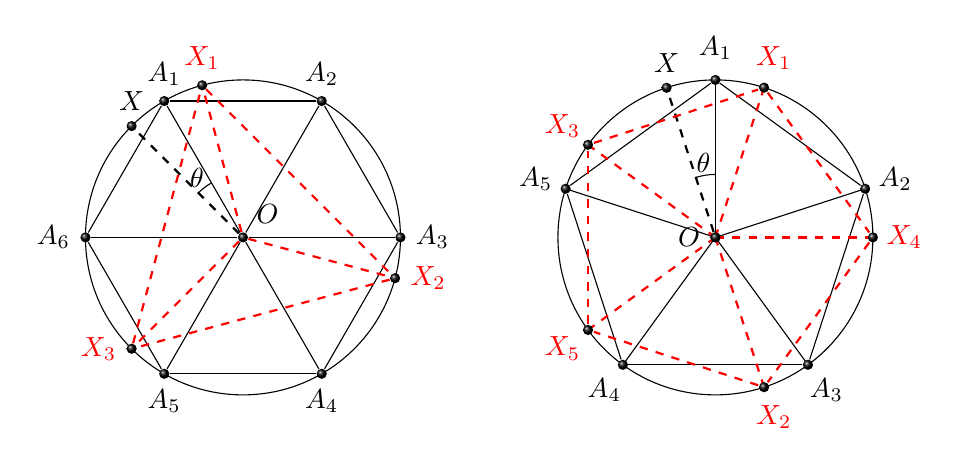
\begin{tikzpicture}
\begin{scope}
    \draw (0,0) circle [radius=2]; %circle
    \node[ball,label={above right:$O$}] (o) at (0,0) {};  %center
    \node[ball,label={above:$X$}] (x) at (-1.414, 1.414) {};    %X
    %original hexagon
    \node[ball,label={above:$A_1$}] (1) at (-1, 1.732) {};
    \node[ball,label={above:$A_2$}] (2) at (1, 1.732) {};
    \node[ball,label={right:$A_3$}] (3) at (2, 0) {};
    \node[ball,label={below:$A_4$}] (4) at (1, -1.732) {};
    \node[ball,label={below:$A_5$}] (5) at (-1, -1.732) {};
    \node[ball,label={left:$A_6$}] (6) at (-2, 0) {};
    \draw (1) to (2);
    \draw (2) to (3);
    \draw (3) to (4);
    \draw (4) to (5);
    \draw (5) to (6);
    \draw (6) to (1);
    \draw (o) to (1);
    \draw (o) to (2);
    \draw (o) to (3);
    \draw (o) to (4);
    \draw (o) to (5);
    \draw (o) to (6);
    %rotated triangle
    \node[ball,label={above, red:$X_1$}] (x1) at (-0.518, 1.932) {};
    \node[ball,label={right, red:$X_2$}] (x2) at (1.932, -0.518) {};
    \node[ball,label={left, red:$X_3$}] (x3) at (-1.414, -1.414) {};
    \draw[dashed, thick] (o) to (x);
    \draw[dashed, red, thick] (o) to (x1);
    \draw[dashed, red, thick] (o) to (x2);
    \draw[dashed, red, thick] (o) to (x3);
    \draw[dashed, red, thick] (x1) to (x2);
    \draw[dashed, red, thick] (x2) to (x3);
    \draw[dashed, red, thick] (x3) to (x1);
    % angle
    \pic [draw,
          angle radius=8mm, angle eccentricity=1.2,
          "$\theta$"] {angle = 1--o--x};
\end{scope}
\begin{scope}[xshift=6cm,scale=2]
    \draw (0,0) circle [radius=1];  %circle
    \node[ball,label={left:$O$}] (o) at (0,0) {};   %center
    \node[ball,label={above:$X$}] (x) at (-0.31,0.95) {};   %X
    \draw[dashed, thick] (o) to (x);
    \def\deg{72}    %interior angle
    %original pentagon
    \foreach [evaluate={
        \t=int(162-\x*\deg);
        }]\x in {1,2,...,5}
    {\draw (0:0)--(\t:1) node[ball] (\x) at (\t:1) {};
    \node[anchor=center] at (\t:1.2) {$A_{\x}$};}
    \foreach \from/\to in {1/2, 2/3, 3/4, 4/5, 5/1}
    {\draw (\from) -- (\to);}
    % angle
    \pic [draw,
          angle radius=8mm, angle eccentricity=1.2,
          "$\theta$"] {angle = 1--o--x};
    %rotated pentagon
    \foreach [evaluate={
        \t=int(144-\x*\deg);
        \p=int(72-2*(\x-1)*\deg);
        }]\x in {1,2,...,5}
    {\draw[dashed, red, thick] (0:0)--(\t:1) node[ball] (\x) at (\t:1) {};
    \node[anchor=center, red] at (\p:1.2) {$X_{\x}$};}
    \foreach \from/\to in {1/2, 2/3, 3/4, 4/5, 5/1}
    {\draw[dashed, red, thick] (\from) -- (\to);}
    \node[ball] at (0,0) {};
\end{scope}
\end{tikzpicture}
\end{document}